\makeatletter
\def\input@path{{../../}}
\makeatother
\documentclass[../../main.tex]{subfiles}

\graphicspath{
	{../../img/}
	{../img/}
	{img/}
}

\begin{document}
\subsection{Независимость КрИ-2 от пути интегрирования}	

Говорят, что КрИ-2 $\int\limits_{\tiny{\overbow{AB}}} P \ dx + Q \ dy$
не зависит от пути интегрирования, если он имеет одну и ту же 
величину для кривой с началом в $A$ и концом в $B$.
(смотри на пример "Физический смысл интегралов"). 

Выражение

\begin{equation}
\label{lec_21, num_1}
P(x,y) \ dx + Q(x,y) \ dy
\end{equation} 

называют полным дифференциалом в некоторой области $D$, если 
$\exists F(x,y),\ (x,y) \in D : dF(x,y) = P(x,y) \ dx + Q(x,y) \ dy$.
Функция $F$ в этом случае называют первообразной для \eqref{lec_21, num_1}.

\begin{thm}[основная теорема о КрИ] 
Пусть в односвязной области $D \subset \R^2$ определены функции $P, Q$,
непрерывные и имеющие непрерывные частные производные $P'_y$ и $Q'_x$.
Тогда следующие 4 условия равносильны: 

\begin{enumerate}[label=\arabic*$^{\circ}$]
	\item Для любого замкнутого контура $L \subset D$ кусочно гладкого:
	
	\[
	\ointctrclockwise\limits_{L} P(x,y) \ dx + Q(x,y) \ dy = 0, \]
	
	\item $\int\limits_{\tiny{\overbow{AB}}} P \ dx + Q \ dy$ не будет 
	зависеть от пути интегрирования $\forall \overbow{AB} \subset D$,
	\item Выражение $P \ dx + Q \ dy$ является полным дифференциалом в $D$,	
	\item В $D$ выполнены условия Эйлера: 
	
	\[ 
	P'_y(x,y) = Q'_x(x,y),\ \forall (x,y) \in D.
	\] 
	
\end{enumerate}
\begin{proof}
Доказательство проведём по следующей схеме: 

\[
1^{\circ} \implies 2^{\circ} \implies 3^{\circ} \implies
4^{\circ} \implies 1^{\circ}
\]

Докажем $1^{\circ} \implies 2^{\circ}$.

Пусть $A$ и $B$ --- любые две точки $D$ и I и II --- пути между $A$ и $B$:

\begin{center}
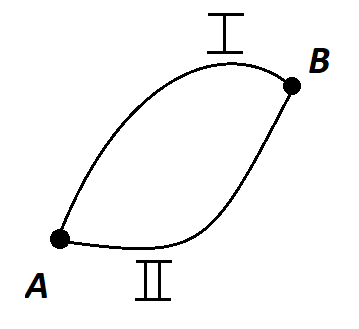
\includegraphics[scale = 0.5]{lec21_1.png}
\end{center}

Тогда контур $A_{I} B_{II}$ --- замкнутый. Значит 

\[
\int\limits_{\tiny{\overbow{A_I B_{II} A}}} P \ dx + Q \ dy = 0
\iff \int\limits_{\tiny{\overbow{A_I B}}} P \ dx + Q \ dy \ +
\int\limits_{\tiny{\overbow{B_{II} A}}} P \ dx + Q \ dy = 0 \iff \]
\[
\iff \int\limits_{\tiny{\overbow{A_I B}}} P \ dx + Q \ dy \ -
\int\limits_{\tiny{\overbow{A_{II} B}}} P \ dx + Q \ dy = 0
\implies \int\limits_{\tiny{\overbow{A_I B}}} P \ dx + Q \ dy \
= \int\limits_{\tiny{\overbow{A_{II} B}}} P \ dx + Q \ dy.
\]

$2^{\circ} \implies 3^{\circ}$.

Зафиксируем какую-либо точку $M_0(x_0, y_0) \in D$. 
Тогда $\forall M(x,y) \in D$ можно определить
$\int\limits_{\tiny{\overbow{M_0 M}}} P \ dx + Q \ dy = F(x,y)$. 
Он зависит только от точки $M_0$, т.~е. от $(x,y)$.

Покажем, что эта функция и является первообразной для \eqref{lec_21, num_1}:

\begin{center}
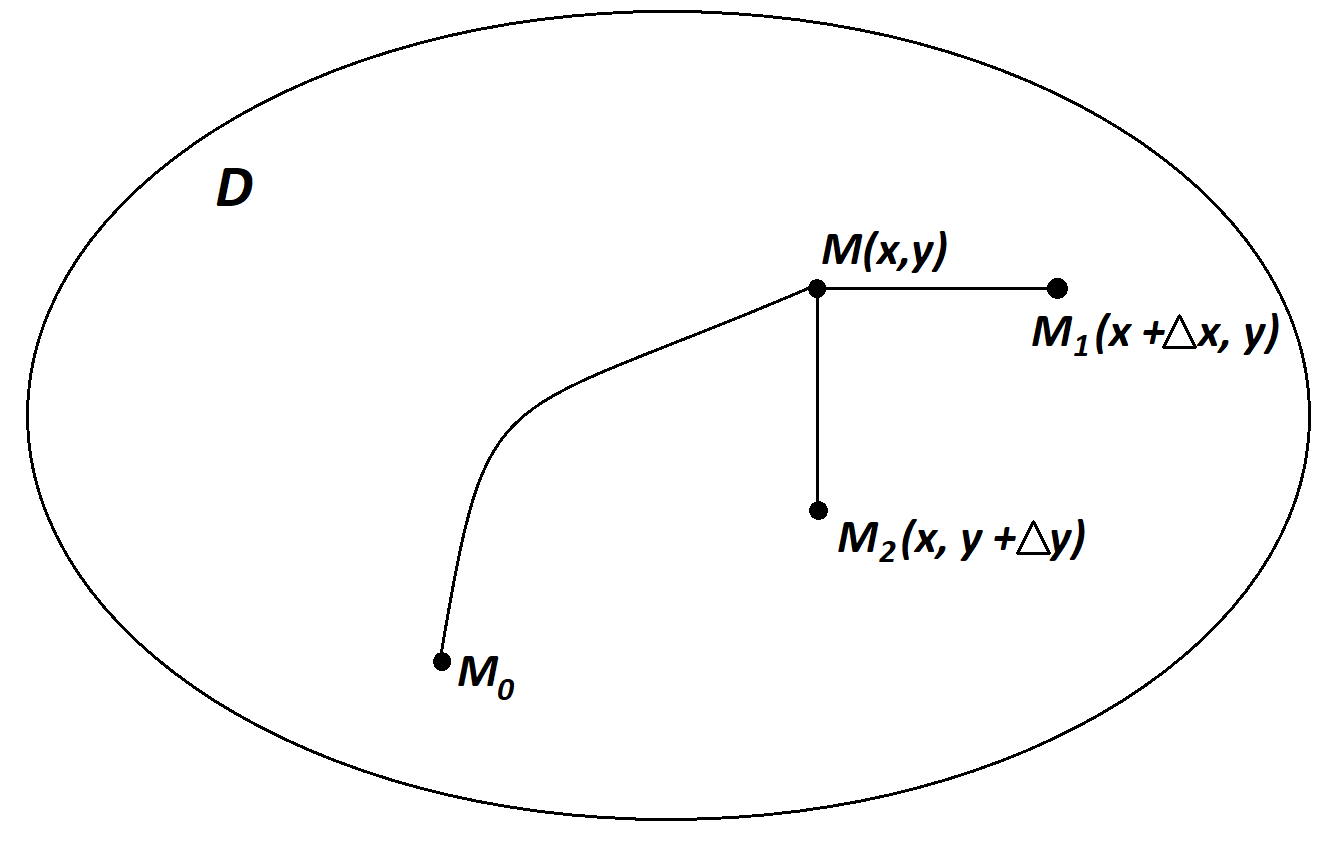
\includegraphics[scale = 0.35]{lec21_2.png}
\end{center}

Придаём приращение $\Delta x$ точке $M$, тогда 

\[
\Delta_x F = F\left(x + \Delta x\right) - F(x) = 
\int\limits_{\tiny{\overbow{M_0 M_1}}} P \ dx + Q \ dy -
 \int\limits_{\tiny{\overbow{M_0 M}}} P \ dx + Q \ dy = \ast
\]

Будем считать, что кривая $M_0 M_1$ состоит из дуги
$\overbow{M_0 M}$ и отрезка $\overline{M M_1}$. Значит

\[
\ast = \int\limits_{\overline{M M_1}} P(x,y) \ dx + Q(x,y) \ dy = \left[ 
\overline{M M_1}: 
\begin{cases} 
y = y = const, \\
x \in [x; x + \Delta x]
\end{cases}
\right] =
\int\limits_{x}^{x + \Delta x} P(x,y) \ dx = \ast
\]

Теорема о среднем:  $\exists \ t \in [x; x + \Delta x] : \ast = P(t,y) \ \Delta x$, 
а тогда $\dfrac{\Delta F}{\Delta x} \appr{\Delta x \to 0} P(x,y)$, 
т.~е. $F'_x = P(x,y)$

Аналогично, если мы придадим приращение $\Delta y$ точке $M$,
т.~е. получим точку $M_2(x, y + \Delta y)$, 
то используя такие же рассуждения получим $F'_y = Q(x,y)$.
А тогда 

\[
dF = F'_x \ dx + F'y \ dy  = P \ dx + Q \ dy 
\]
Что и требовалось доказать.

$3^{\circ} \implies 4^{\circ}$

$P \ dx + Q \ dy = dF$, т.~е. $F'_x = P$, а $F'_y = Q$.

Тогда $F''_{xy} = P'_y, F''_{yx} = Q'_x \implies 
\left[  
\text{теорема о равенстве смешанных производных}
\right] 
\implies 
\implies F'_y = Q'_x$

$4^{\circ} \implies 1^{\circ}$

Возьмём гладкий контур $L \subset D$. 
Пусть он ограничивает область $G \subset D$, тогда по формуле Грина

\[
\ointctrclockwise\limits_{L} P \ dx + Q \ dy = 
\iint\limits_{G} (Q'_x - P'_y) dx dy = 
\iint\limits_{G} 0 dx dy = 0
\]
\end{proof}
\end{thm}

\subsection{Вычисление первообразной}

Пусть в области $D$ выполнены условия Эйлера. 
Значит существует первообразная для $P \ dx + Q \ dy$.
$F(x,y) = \int\limits_{(x_0,y_0)}^{(x,y)} P \ dx + Q \ dy$.

Здесь: 
интеграл не зависит от пути интегрирования. 
В таких случаях интеграл
$\int\limits_{\tiny{\overbow{AB}}} P \ dx + Q \ dy$ принято записывать
$\int\limits_{A}^{B} P \ dx + Q \ dy$

В простейших случаях функцию $F(x,y)$ можно найти так:

\begin{center}
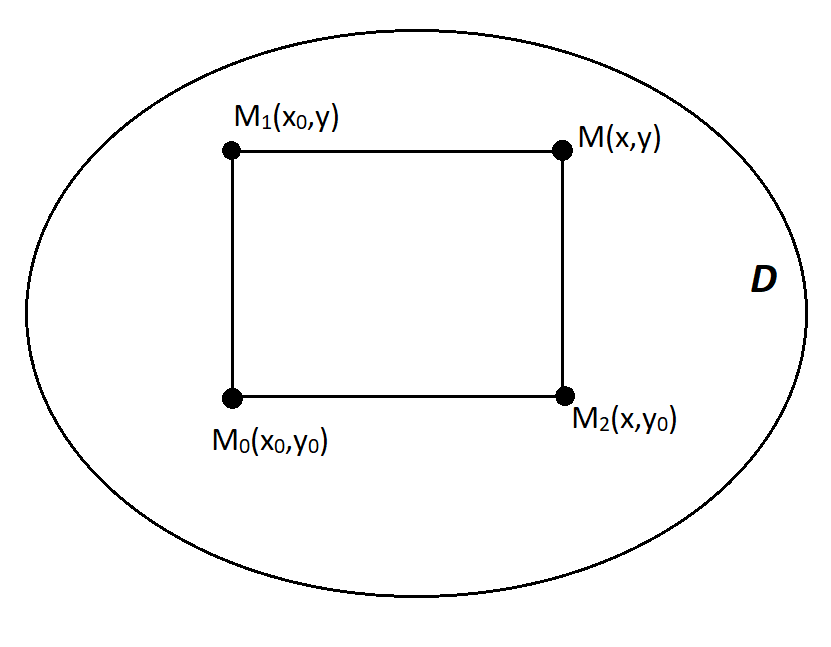
\includegraphics[scale = 0.5]{lec21_3.png}
\end{center}

\[
F(x,y) = \int\limits_{\overline{M_0 M_1}} P \ dx + Q \ dy \ +
\int\limits_{\overline{M_1 M}} P \ dx + Q \ dy
= \ast
\]

В первом интеграле $x = const,\ dx = 0,\ y \in [y_0; y]$.
Во втором $y = const,\ dy = 0,\ x \in [x_0;x]$. Тогда:

\[
\ast = \int\limits_{y_0}^{y} Q(x_0, y) \ dy +
\int\limits_{x_0}^{x} P(x,y) \ dx
\]

Таким образом 

\[
F(x,y) = \int\limits_{x_0}^{x} P(x,y) \ dx + \int\limits_{y_0}^{y} Q(x_0, y) \ dy 
\]

Здесь $(x_0,y_0)$ --- любая точка области.

Если в качестве кривой $M_0 M$ взять $\overbow{M_0 M_2 M}$, то получим 

\[
F(x,y) = \int\limits_{y_0}^{y} Q(x, y) \ dy +
\int\limits_{x_0}^{x} P(x,y_0) \ dx
\]

\subsection{Использование первообразной для вычисления интегралов}

Пусть в $D$ выполнены условия Эйлера и рассматриваем интеграл

\[
\int\limits_{\tiny{\overbow{AB}}} P(x,y) \ dx + Q(x,y) \ dy = \ast
\]

Заменим $\overbow{AB}$, если нужно, гладкой кривой
$
\begin{cases} x = x(t), 
\\ y = y(t), 
\\ \alpha \leq t \leq \beta 
\end{cases}$,
у которой 
$
\begin{cases} 
(x(\alpha), y(\alpha) \longleftrightarrow A, \\
(x(\beta), y(\beta)) \longleftrightarrow B;
\end{cases}
$, тогда

\[
\ast = 
\int\limits_{\alpha}^{\beta}(
P(x(t), y(t)) \ x'(t) +
Q(x(t), y(t)) \ y'(t)
) \ dt = 
\int\limits_{\alpha}^{\beta} F'_t(x(t), y(t)) \ dt =
F(x(t), y(t)) \bigg|_{\alpha}^{\beta} =
\]
\[
= F(x(\beta), y(\beta)) - F(x(\alpha), y(\alpha)) = 
F(x,y) \bigg|_A^B
\] 

То есть 
$\int\limits_{\tiny{\overbow{AB}}} P \  dx + Q \ dy =
F(x,y) \bigg|_A^B$

\begin{example}
$I = \int\limits_{\tiny{\overbow{AB}}} 2xy \ dx + x^2 \ dy,\
A(1,0),\ B(10,2)$.

$P'_y = 2x,\ Q'_y = 2x$

Выполнены условия Эйлера. Найдём первообразную 

\[
F(x,y) = \int\limits_{x_0}^{x} P(x,y) \ dx +
\int\limits_{y_0}^{y} Q(x_0, y) \ dy = 
\left[ 
(x_0,y_0) = (0,0)  
\right] =
\int\limits_{0}^{x} 2xy \ dx + 
\int\limits_{0}^{y} 0 \ dy = 
\int\limits_{0}^{x} 2xy \ dx = 
x^2y
\]
\[
I = x^2y \bigg|_{(1,0)}^{(10,2)} = 200
\]
\end{example}
\end{document}